\documentclass[a4paper,landscape]{article}

\usepackage[utf8]{inputenc}
\usepackage[T1]{fontenc}
\usepackage[ngerman]{babel}
\usepackage[page]{totalcount}

\usepackage{geometry}
\usepackage{titlesec}
\usepackage{fancyhdr}

\usepackage{amsmath}
\usepackage{amssymb}

\usepackage{listings}
\usepackage{enumitem}

\usepackage{tikz}
\usetikzlibrary{automata, positioning, arrows}

\usepackage{graphicx}
\usepackage{tabularx}

\usepackage{multicol}

\DeclareUnicodeCharacter{0308}{~}
\hyphenation{
	prak-tisch
	un-mög-lich
}

% rotate page and set margins %
\geometry{left=0.55cm,right=0.55cm,top=1.10cm,bottom=0.55cm,landscape,headsep=2mm}

% make header and footer %
\pagestyle{fancy}
\fancyhead{} % clear header
\fancyhead[L]{Zusammenfassung Informationssicherheit}
\fancyhead[R]{\thepage\hspace{1mm}von\hspace{1mm}\totalpages} 
\fancyfoot{} % clear footer

% configure document %
\setlist{itemsep=1pt,parsep=0pt}
\setlength{\parindent}{0pt}
\setlength{\parskip}{0pt}
\setlength{\topskip}{10pt}
\setlength{\columnseprule}{0.5pt} % column seperator line

% change style %
\titleformat*{\section}
{\large\bfseries} 
\titlespacing*{\section}
{0pt}{4pt}{0pt}

\titleformat*{\subsection}
{\normalsize\bfseries}
\titlespacing*{\subsection}
{0pt}{4pt}{0pt}

\titleformat*{\subsubsection}
{\normalsize\bfseries}
\titlespacing*{\subsubsection}
{0pt}{4pt}{0pt}

\titleformat*{\paragraph}
{\normalsize\bfseries}
\titlespacing{\paragraph}
{0pt}{.5em}{.5em}

\titleformat*{\subparagraph}
{\small\bfseries}
\titlespacing{\subparagraph}
{0pt}{.5em}{.5em}

\title{Zusammenfassung Informationssicherheit} 
\author{Louis Seubert}

\newcommand{\ord}{\operatorname{ord}}

\newcommand{\N}{\ensuremath{\mathbb{N}}}
\newcommand{\No}{\ensuremath{\mathbb{N}_0}}
\newcommand{\Z}[1]{\ensuremath{\mathbb{Z}_{#1}}}
\newcommand{\Zx}[1]{\ensuremath{\mathbb{Z}_{#1}^{*}}}

\newcommand{\calO}{\ensuremath{\mathcal{O}}}

\newcommand{\plaint}{\ensuremath{m}}
\newcommand{\ciphert}{\ensuremath{c}}
\newcommand{\signiture}{\ensuremath{s}}

\newcommand{\skey}{\ensuremath{sk}}
\newcommand{\pkey}{\ensuremath{pk}}

\newcommand{\enc}{\textsc{Enc}}
\newcommand{\dec}{\textsc{Dec}}
\newcommand{\sig}{\textsc{Sig}}
\newcommand{\ver}{\textsc{Ver}}

\newenvironment{definitions}{
	\par\vspace{\abovedisplayshortskip}\noindent
	\tabularx{\columnwidth}{>{$}l<{$} @{${}={}$} >{\raggedright\arraybackslash}X}
}{\endtabularx\par\vspace{\belowdisplayshortskip}}

\begin{document}
\begin{multicols*}{4}
	\section{Grundlagen}
	\subsection*{Allgemeines}
	\[
		x^{k} \bmod p \equiv \left( x \bmod p \right)^{k \bmod \varphi(p)} \bmod p
	\]
	\[
		\gcd(a,m) = 1 \Rightarrow a^{\varphi(m)} \equiv 1 \bmod m
	\]

	\subsection*{Berechnung der Stellenzahl}
	Die Anzahl \(a\) der Ziffern der \(b\)-adischen Darstellung einer natürlichen
	Zahl \(n \in \No\) berechnet sich wie folgt:
	\[
		a =
		\begin{cases}
			1,                               & \quad \text{wenn } n = 0    \\
			\lfloor \log_{b}{n} \rfloor + 1, & \quad \text{wenn } n \geq 1
		\end{cases}
	\]

	\subsection*{Teilbarkeit}
	Zwei Zahlen \(a,b \in \mathbb{Z}\) werden als teilerfremd bezeichnet, wenn
	\(\gcd(a,b) = 1\) ist.

	\subsection*{Ordnung}
	Die Ordnung eines Gruppenelementes \(g\) einer Gruppe \((G,\cdot)\) ist die
	kleinste natürliche Zahl \(n > 0\) für die gilt \(g^{n} = e\), wobei \(e\)
	das neutrale Element der Gruppe ist.
	\paragraph*{Multiplikative Ordnung} \(\ord_{m}(a)\) ist die multiplikative
	Ordnung modulo \(m\) des Elementes \(a\), d.h. der kleinste positive Exponent
	\(n\) für den gilt: \[x^{n} \equiv 1 \pmod{m}\] Eine Erweiterung dessen ist:
	\[\ord(x^{l}) = \frac{\ord(x)}{\gcd(\ord(x),l)}\]
	\paragraph*{Primzahlen} Die Ordnung für Primzahlen lässt sich wie folgt
	bestimmen: \[\ord(p) = \varphi(p) = p -1 \]

	\subsection{Multiplikative Inverse}
	Das Multiplikative Inverse von \(a\) im Modul \(m\) lässt sicht mit dem
	erweiterten euklidischen Algorithmus berechnen. Der Algorithmus liefert die
	Linearkombination
	\[\gcd(a,m) = u \cdot a + v \cdot m = 1\]
	wenn \(a\) und \(m\) teilerfremd sind. Somit lässt sich das Inverse dann
	einfach ablesen:
	\[a^{-1} \equiv u \bmod m\]

	\subsection{Eulersche Phi-Funktion}
	Die Eulersche Phi-Funktion gibt an, wie viele ganze Zahlen teilefremd zu
	\(n\) sind. Wenn \(p\) eine Primzahl ist dann kann man folgende aussagen
	treffen:
	\[\varphi(p) = p - 1\]
	\[\varphi(p^{k}) = p^{k-1} \cdot \left(p - 1\right)\]
	\[\varphi(n \cdot m) = \varphi(n) \cdot \varphi(m)\]
	\[\varphi(n) = n \prod_{p|n} \left(1 - \frac{1}{p}\right)\]
	Wobei \(p|n\), die Primfaktoren der Zahl \(n\) sind.


	\subsection{Kontravalenz}
	\begin{center}
		\begin{tabular}{c| c c }
			$\oplus$ & 0 & 1 \\ \hline
			0        & 0 & 1 \\
			1        & 1 & 0
		\end{tabular}
	\end{center}

	\subsection{Diskreter Logarithmus}
	Der diskrete Logarithmus ist die kleinste Lösung für \(x\) der Gleichung
	\(a^{x} \equiv m \bmod p$ mit $m,\;a \in\mathbb{N},\;p \in\mathbb{Z}_{p}\). \par
	Da sich die diskrete Exponentiation leicht berechnen lässt, gilt das nicht
	für die Umkehrfunktion. \emph{(Diffie-Hellman-Annahme)} Aufgrund dessen wird
	diese "Einwegfunktion" u. a. im Diffie-Hellman-Key-Exchange,
	der ElGamal-Encryption und vielem mehr eingesetzt. Jedoch ist diese Funktion
	ungeignet für Verschlüsselungsmethoden, da es keine "Falltür" zum
	entschlüssel gibt.

	\subsection{Modulares Potenzieren}
	Seien \(x,k,m \in\mathbb{N}\), gesucht ist \(z = x^{k} \bmod m\)
	\begin{enumerate}
		\item Binärdarstellung von \(k\)
		\item Ersetzen jeder \(0\) durch \textbf{Q} und jeder \(1\) durch
		      \textbf{QM}
		\item Dabei wird \textbf{Q} als Anweisung zum \emph{Quadrieren} und
		      \textbf{M} als Anweisung zum \emph{Multiplizieren} mit der Basis \(x\)
		      aufgefasst.
		\item Begonnen wird mit 1 bzw. kann die erste \textbf{QM} Anweisung
		      durch \(x\) substituiert werden.
	\end{enumerate}

	\subsection{Chinesischer Restsatz}
	Seien \(m_{1}, \ldots, m_{n} \in\mathbb{N}\) paarweise teilerfremd, dann hat
	das System von Kongruenzen eine eindeutige Lösung \(x \in \mathbb{Z}_{m}\),
	wobei \(m = m_{1} \cdot \ldots \cdot m_{n}\) das Produkt der einzelnen Module
	ist. \[x \equiv a_{1} \bmod m_{1}, \;\ldots, x \equiv a_{n} \bmod m_{n}\]
	Eine Lösung $x$ kann wie folgt ermittelt werden:
	\[x = \left( \sum_{i = 1}^{n} a_{i} \cdot M_{i} \cdot N_{i} \right) \bmod m\]
	mit folgenden Vorraussetztungen:
	\begin{definitions}
		$$m$$ & $m = m_{1} \cdot \ldots \cdot m_{n}$ \\
		$$M_{i}$$ & $\frac{m}{m_{i}}$ \\
		$$N_{i}$$ & $M_{i}^{-1} \bmod m_{i}$
	\end{definitions}

	\subsection{Euklidischer Algorithmus}
	Setze $r_{0} := a, r_{1} := b$
	\begin{eqnarray*}
		r_{0} &=& q_2 \cdot r_{1} + r_{2} \\
		r_{1} &=& q_3 \cdot r_{2} + r_{3} \\
		&\vdots& \\
		r_{n-2} &=& q_{n} \cdot r_{n-1} + r_{n} \\
		r_{n-1} &=& q_{n+1} \cdot r_{n} + 0
	\end{eqnarray*}
	\paragraph{Erweiterung}
	{\small
		\begin{align*}
			x_{0} & = 1 \quad x_{1} = 0             & y_{0} & = 0 \quad y_{1} = 1             \\
			x_{2} & = x_{0} - q_{2} \cdot x_{1}     & y_{2} & = y_{0} - q_{2} \cdot y_{1}     \\
			x_{3} & = x_{1} - q_{3} \cdot x_{2}     & y_{3} & = y_{1} - q_{3} \cdot y_{2}     \\
			x_{n} & = x_{n-2} - q_{n} \cdot x_{n-1} & y_{n} & = y_{n-2} - q_{n} \cdot y_{n-1}
		\end{align*}}
	dann gilt $x_{n}a + y_{n}b = \gcd(a,b)$.

	\subsection{Primitivwurzeln}
	Eine ganze Zahl \(a\) ist eine Primitivwurzel modulo \(m\) wenn gilt dass
	die Ordnung von \(a\) modulo \(m\) gleich der Gruppenordnung der primen
	Restklassengruppe ist: \[\ord_m(a)=\varphi(m)\]

	\paragraph{Primitivwurzeltest} Um festzustellen, ob eine Zahl \(g\) eine
	Primitivwurzel in der Restklassengruppe \(\mathbb{Z}_{p}^{*}\) mit \(p\) ist
	Primzahl ist, führe man folgende Schritte aus:
	\begin{enumerate}
		\item Primfaktorzerlegung von \(p-1\):\par
		      \(p-1 = p_{1} \cdot \ldots \cdot p_{i}\)
		\item Prüfe für alle \(q \in \{p_{1},\ldots, p_{i}\}\) ob gilt
		      \(g^{(p-1)/q} \not\equiv 1 \pmod p\) \par
		\item Sollten demnach alle Primfaktoren ungleich \(1 \bmod p\) sein, dann
		      ist \(g\) eine Primitivwurzel.
	\end{enumerate}

	Falls \(g\) eine Primitivwurzel von \(\mathbb{Z}_{p}^{*}\) ist, dann ist auch
	\(a = g^{t}\) eine Primitivwurzel von \(\mathbb{Z}_{p}^{*}\) genau dann wenn
	gilt: \(\gcd(t,\varphi(p)) = 1\). Somit lässt sich folgendes aussagen:
	\[\gcd(t,\varphi(p)) = 1 \Rightarrow \langle g^{t} \rangle = \mathbb{Z}_{p}^{*}\]

	\subsection{Miller-Rabin}

	\section{Verschlüsselungsalgorithmen}
	\subsection{Asymetrische Verfahren}

	\subsubsection{RSA}
	\paragraph{Schlüsselerzeugung}
	\begin{enumerate}
		\item Wähle zwei große Primzahlen \(p, q\) mit \(p \neq q\) und
		      vorgegebener Bitlänge \(k\).
		\item Berechne \(n = p \cdot q\).
		\item Berechne \(\varphi(n) = (p - 1)(q - 1)\)
		\item Wähle \(e \in \{3, \dotsc, \varphi(n) - 1\}\), wobei
		      \(\gcd(e, \varphi(n)) = 1\).
		\item Berechne mit Hilfe des erweiterten Euklid das zu \(e\)
		      multiplikativ-inverse Element \(d\) bezüglich
		      \(\varphi(n)\): \par
		      \(\gcd(e,\varphi(n)) = 1 = e \cdot d + k \cdot \varphi(n)\)
		\item \((\pkey, \skey) \leftarrow ((n,e), (n,d))\).
	\end{enumerate}

	\paragraph{Verfahren}
	\begin{align*}
		\enc(\pkey,\plaint)        & = \plaint^{e} \bmod n                               \\
		\dec(\skey,\ciphert)       & = \ciphert^{d} \bmod n                              \\
		\sig(\skey,\plaint)        & = \plaint^{d} \bmod n                               \\
		\ver(\pkey,\plaint,\sigma) & = 1 :\;\Leftrightarrow \plaint = \sigma^{e} \bmod n
	\end{align*}

	\paragraph{Verschlüsselung mit RSA-OAEP}
	Die RSA-OAEP (\emph{optimal asymmetric encryption padding}) Variante ist
	gegen deterministische Angriffe sicher! Die Funktionen \(g(x)\) und \(h(x))\)
	sind Hashfunktionen.

	\subparagraph{Verschlüsselung}
	\begin{enumerate}
		\item Wähle \(r\) zufällig
		\item Berechne \par
		      \(x = m \oplus g(r)\) und \(y = r \oplus h(x)\)
		\item Verschlüssele \par
		      \(\enc_{\text{OAEP}}(\pkey,\plaint) = (x||y)^{e} \bmod n\)
	\end{enumerate}

	\subparagraph{Entschlüsselung}
	\begin{enumerate}
		\item Rekonstruiere \((x||y) = \dec(\skey,\ciphert)\)
		\item Rekonstruiere \(r\) mit \(r = y \oplus h(x)\)
		\item Berechne \plaint mit \(\plaint = x \oplus g(r)\)
	\end{enumerate}

	\paragraph{Signieren und Entschlüsseln mit dem Chinesischen Restsatz}
	\[
		i =
		\begin{cases}
			c & \text{für Entschlüsseln} \\
			m & \text{für Signieren}
		\end{cases}
	\]
	\[
		o =
		\begin{cases}
			m & \text{für Entschlüsseln} \\
			s & \text{für Signieren}
		\end{cases}
	\]
	\begin{enumerate}
		\item $d_{p} = d \bmod (p-1) \;,\; d_{q} = d \bmod (q-1)$
		\item $i_{1} = i^{d_{p}} \bmod p \;,\; i_{2} = i^{d_{q}} \bmod q$
		\item \(
		      h =
		      \begin{cases}
			      q^{-1} \cdot (i_{1} - i_{2})     & \text{falls } i_{1} > i_{2} \\
			      q^{-1} \cdot (i_{1} - i_{2} + p) & \text{falls } i_{1} < i_{2}
		      \end{cases}
		      \)
		      \
		\item $h = h \bmod p$
		\item $o = i_{2} + (h \cdot q)$
	\end{enumerate}

	\subsubsection{ElGamal}
	\paragraph{Schlüsselerzeugung}
	\begin{enumerate}
		\item Wähle eine große Primzahlen \(p\) mit vorgegebener Bitlänge \(k\)
		\item Suche eine Primitivwurzel \(g\) in der Gruppe \(\mathbb{Z}_{p}\)
		\item Wähle einen zufälligen Exponenten \(x \in\{2,\ldots,\;p-2\}\)
		\item Berechne \(y = g^{x} \bmod p\)
		\item \((\pkey,\skey) \leftarrow ((p,g,y),(p,g,x))\)
	\end{enumerate}

	\paragraph{Verfahren} \,\\
	\(k \in\{1,\ldots,p-2\}\) wird für jedes Verfahren erneut zufällig gewählt.
	\begin{align*}
		\enc(\pkey,\plaint)          & = \left((g^{k}),(y^{k} \cdot \plaint)\right) \pmod p \\
		\dec(\skey,(g^{k},\ciphert)) & = (g^{k})^{p-1-x} \cdot \ciphert \pmod p             \\
		\sig(\skey,\plaint)          & = (s_{1},s_{2})                                      \\
		\ver(\pkey,\plaint,\sigma)   & = 1 :\;\Leftrightarrow v_{1} = v_{2}
	\end{align*}

	Für \sig\ gilt zudem dass \(\gcd(k,p-1) = 1\)
	\begin{align*}
		s_{1} & := g^{k} \bmod p                                  \\
		s_{2} & := k^{-1} \cdot (\plaint - a \cdot x) \bmod (p-1)
	\end{align*}

	Für \ver\ gilt zudem dass \(1 \leq s_{1} \leq p-1\)
	\begin{align*}
		v_{1} & := g^{\plaint} \bmod p                   \\
		v_{2} & := y^{s_{1}} \cdot s_{1}^{s_{2}} \bmod p
	\end{align*}

	\subsection{Symmetrische Verfahren}
	\subsubsection{DES}
	\begin{center}
		\begin{tabular*}{.9\linewidth}{r|l@{\extracolsep{\fill}}}\hline
			Struktur & Feistelchiffre    \\\hline
			Schlüssellänge & 56 Bit      \\\hline
			Blocklänge & 64 Bit          \\\hline
			Rundenanzahl & 16            \\\hline
		\end{tabular*}
	\end{center}

	\subsubsection{AES}
	\begin{center}
		\begin{tabular*}{.9\linewidth}{r|l@{\extracolsep{\fill}}}\hline
			Struktur & Substitutionschiffre          \\\hline
			Schlüssellänge & 128, 192 oder 256 Bit   \\\hline
			Blocklänge & 128 Bit                     \\\hline
			Rundenanzahl & 10, 12 oder 14            \\\hline
		\end{tabular*}
	\end{center}

	\subsection{Blockverschlüsselung}
	\begin{center}
		\begin{tabular}{c | c}
			\textbf{Blockorientiert} & \textbf{Stromorientiert} \\\hline
			ECB                      & OFB                      \\
			CBC                      & CFB
		\end{tabular}
	\end{center}
	Stromorientierte Betriebsarten erfordern kein Padding das Klartextes, und
	unterstützen keine asymetrische Verschlüsselung. \par
	Um einen Klartext \plaint verschlüsseln zu können muss diser in Blöcke der
	Länge $r \leq n$ eingeteilt werden. Dabei ist $n$ die Blocklänge des
	Verschlüsselungsverfahren, $r$ die Länge der Klartextblöcke. $\plaint_i$
	bezeichnet dabei einen Block des Klartextes \plaint.

	\subsubsection{ECB}
	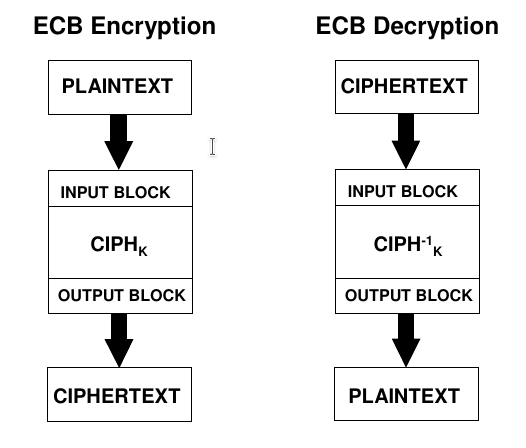
\includegraphics[width=0.2\textwidth]{./images/ecb_mode.png}
	\subsubsection{CBC}
	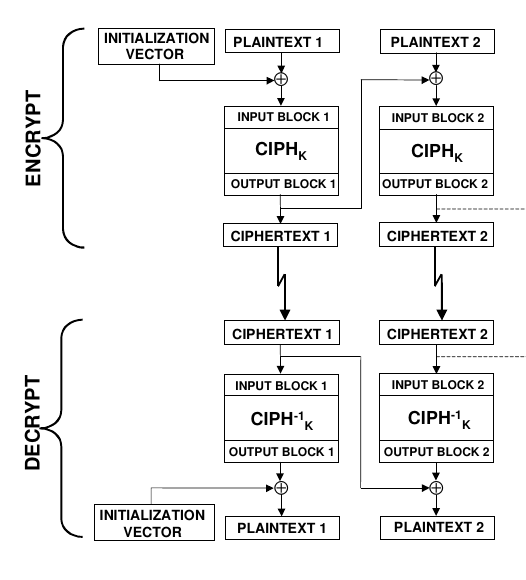
\includegraphics[width=0.2\textwidth]{./images/cbc_mode.png}
	\subsubsection{CFB}
	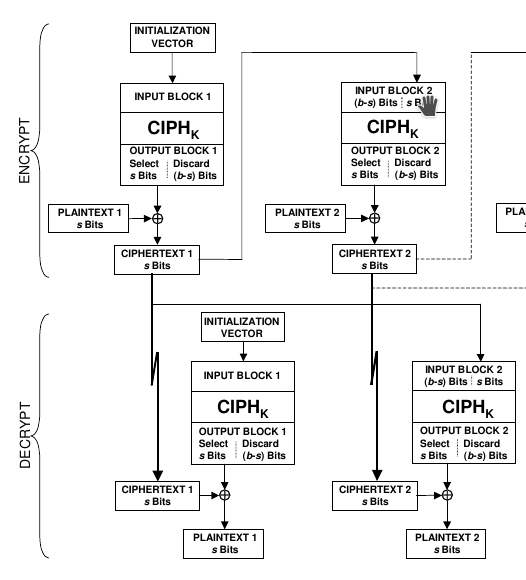
\includegraphics[width=0.2\textwidth]{./images/cfb_mode.png}
	\subsubsection{OFB}
	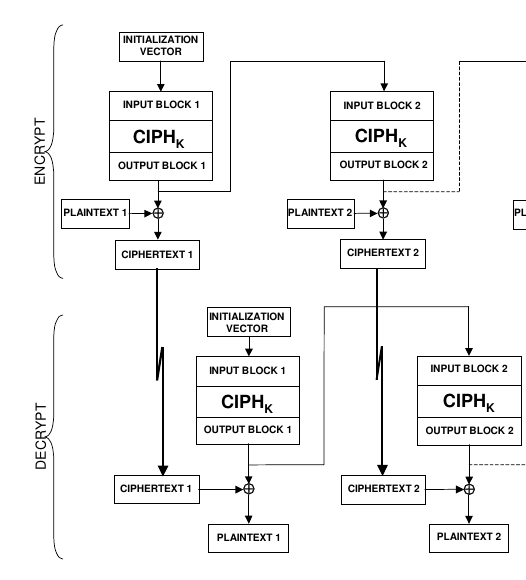
\includegraphics[width=0.2\textwidth]{./images/ofb_mode.png}

	\section{Angriffe gegen Verschlüsselungsalgorithmen}
	\subsection{RSA}
	\subsubsection*{Common-Modulus-Attack}
	Möglich wenn die selbe Nachricht mit zwei unterschiedlichen Exponenten verschlüsselt wird,
	jedoch die Primfaktoren identisch sind. Die beiden Exponent sind dabei jedoch teilerfremd
	zu einander sind.
	\begin{center}
		\begin{tabular}[t]{ccc}
			\pkey        & \ciphert                    & \plaint \\\hline
			$(n, e_{1})$ & $c_{1} = m^{e_{1}} \bmod n$ & $m$     \\
			$(n, e_{2})$ & $c_{2} = m^{e_{2}} \bmod n$ & $m$     \\\hline
		\end{tabular}
	\end{center}
	\begin{enumerate}
		\item Berechne mit dem erweitertem Euklid $a \cdot e_{1} + b \cdot e_{2} = 1$. \par
		      $a$ oder $b$ wird negativ sein.
		\item Berechne nun folgendes:
		      \begin{align*}
			      m & = m^{1}                                                                                           \\
			        & = m^{a \cdot e_{1} + b \cdot e_{2}} = \left(m^{e_{1}}\right)^{a} \cdot \left(m^{e_{2}}\right)^{b} \\
			        & = \left(c_{1}\right)^{a} \cdot \left(c_{2}\right)^{b} \bmod n
		      \end{align*}
		\item Der negative Exponent kann nun auch wie folgt geschrieben werden: \par
		      $x^{-2} = \left(x^{-1}\right)^{2}$ wobei $x^{-1}$ dem Inversen entspricht.
		\item Sollte es kein Inverses geben (d.h. $\gcd(c_{1|2},m) \neq 1$) dann lassen
		      sich die Primfaktoren wie folg berechnen: \par
		      \(
		      n = \underbrace{\gcd(c_{(1|2)},m)}_{p} \cdot \underbrace{\frac{n}{p}}_{q}
		      \)
	\end{enumerate}

	\subsubsection*{Low-Encryption-Exponent-Attack}
	Möglich bei einem kleinen Abstand zwischen den Primfaktoren von \(n\).
	\begin{enumerate}
		\item \(x = \left\lceil\sqrt{n}\right\rceil\)
		\item \(y = \sqrt{x^{2}-n}\)
		\item \(
		      \begin{cases}
			      \text{gehe zu 2} & \text{wenn } y \textbf{ nicht}\text{ ganzzahlig} \\
			      \text{gehe zu 4} & \text{wenn } y \text{ ganzzahlig}
		      \end{cases}\)
		\item \(p = x+y, q = x-y\)
	\end{enumerate}

	\subsubsection*{Small-Message-Space-Attack}
	Wenn die Anzahl der möglichen Nachrichten klein ist und der mögliche Inhalt
	im Vorraus bekannt ist, dann kann der Angreifer eine Liste führen, in welcher
	die möglichen Nachrichten zusammen mit dem \pkey verschlüsselten Nachricht
	aufgeführt werden. Sollte dann eine Nachricht abgefangen werden, muss lediglich
	in der Liste gesucht werden. \par
	Durch den Einsatz von OAEP (Optimal Asymmetric Enrcyption Padding) kann dies
	verhindert werden.

	\subsection{ElGamal}
	\subsubsection*{Berechnungen}
	\subsubsection*{Existenzielles Fälschen}


	\section{Hashfunktionen}
	Eine Hashfunktion ist eine Abbildung welche einen belibig lange Zeichenfolge auf eine
	Zeichenfolge mit fester länge minimiert.
	Eine Hashfunktion kann folgende Eigenschaften besitzen:
	\begin{description}
		\item[Einwegfunktion] \emph{preimage resistance}\par
		      Es ist praktisch unmöglich, zu einem gegebenen Ausgabewert $y$ einen Eingabewert $x$ zu finden,
		      den die Hashfunktion auf $y$ abbildet: $h(x) = y$.
		\item[Kollisionsresistenz]
		      \begin{description}
			      \item[]
			      \item[Schwache] \emph{2nd-preimage resistance}\par
			            Es ist praktisch unmöglich, für einen gegebenen Wert $x$ einen davon verschiedenen Wert
			            $x'$ zu finden, der denselben Hashwert ergibt: $h(x)=h(x')\;,\; x \ne x'$.
			      \item[Starke] \emph{collision resistance}\par
			            Es ist praktisch unmöglich, zwei verschiedene Eingabewerte $x$ und $x'$ zu finden, die
			            denselben Hashwert ergeben.
		      \end{description}
	\end{description}

	\subsection{Message Authentification Codes}
	\emph{Message Authentication Codes} (MACs) sind ein symmetrisches Verfahren,
	um die Authentizität einer Nachricht sicherzustellen. Hierzu gibt es einen
	Signatur- und einen Verifikationsalgorithmus.
	\subsubsection{Hash-MAC}
	Um einen HMAC \(\sigma\) zu prüfen, erstellt der Empfänger selbst einen HMAC
	und prüft, ob diese identisch ist zu \(\sigma\). \par
	\(\textit{opad} = \text{0x5C} \quad \textit{ipad} = \text{0x36}\)
	\[\sig(k,\plaint) = h((k \oplus \textit{opad})|| h((k \oplus\textit{ipad})|| m))\]

	\subsection{Gebrochene Algorithmen}
	\begin{center}
		\begin{tabular}{c| c }
			Algorithmus & Gebrochene Eigenschaft \\ \hline
			MD5         & collision resistance   \\
			SHA-1       & collision resistance
		\end{tabular}
	\end{center}

	\section{Protokolle}
	\subsection{Diffie-Hellman-Schlüsselaustausch}
	Alice und Bob haben einen gemeinsamen öffentlichen Schlüssel $(p,g)$, wobei
	$p$ eine Primzahl ist und $g$ eine Primitivwurzel von \Z{p}.
	\begin{enumerate}
		\item Alice wählt zufälliges $a \in [0;p-2]$ und berechnet $c = g^a \bmod p$
		      und übermittelt $c$ an Bob.
		\item Bob wählt zufälliges $b \in [0;p-2]$ und berechnet $d = g^b \bmod p$
		      und übermittelt $d$ an Alice.
		\item Alice berechnet nun $k = d^a \bmod p$
		\item Bob berechnet nun $k = c^b \bmod p$
	\end{enumerate}

	\subsection{Station-to-Station-Protokoll}
	Eine Erweiterung des Diffie-Hellman-Schlüsselaustausch um einen
	Man-in-the-Middle-Angriff auszuschließen.
	\begin{enumerate}
		\item Alice wählt zufälliges $a \in [0;p-2]$ und berechnet $c = g^{a} \bmod p$
		      und übermittelt $c$ an Bob.
		\item Bob wählt zufälliges $b \in [0;p-2]$ und berechnet $k = g^{ab} \bmod p$
		\item Bob sendet nun $g^{b}$ sowie $z = \enc_{k}(s)$ mit $s = \sig_{\skey_{B}}(g^{a}||g^{b})$
		\item Alice $k = g^{ab} \bmod p$ und $s = \dec_{k}(z)$ sowie $\ver((g^{a}||g^{b}),s,\pkey_{B})$
		\item Alice sendet nun $z = \enc_{k}(s)$ mit $s = \sig_{\skey_{A}}(g^{b}||g^{a})$
		\item Bob entschlüsselt $s = \dec_{k}(z)$ und verifiziert $\ver((g^{b}||g^{a}),s,\pkey_{A})$
	\end{enumerate}
	Sollte die letzte Überprüfung korrekt sein, dann ist ein gemeinsamer Schlüssel gewählt.

\end{multicols*}
\end{document}
